
\subsubsection{Effective temperature models}
\label{sect:irtf-teff}

Table \ref{tab:irtf-teff-rmse} summarises the RMSE/RMDSE for the
complete set of models: the minimum $\chi^2$ estimate based on the
full spectrum ($\chi^2$), the projection pursuit regression based on
the ICA components (PPR-ICA) and models trained on the spectral
features proposed by the GA (GA-RF, GA-GBM, GA-SVR, GA-NNET, GA-MARS,
GA-KPLS, GA-RR). For each model, we report the RMSE/RMDSE obtained for
several noise levels of the training sets.  SNR=$\infty$ corresponds
to noiseless spectra. In the GA-cases, the model is trained with the
spectral features found by the Genetic Algorithms when applied to
BT-Settl spectra of the corresponding SNR.

Table \ref{tab:irtf-teff-rmse} shows that the performance of classifiers
based on the full spectrum (or in a compressed version in the form of
ICA components) and the best classifier based on features derived from
limited spectral bands is equivalent. The Bartlett test shows that the
variances are homogeneous with a Bartlett\textquoteright s K-squared
of 8.5 with 2 degrees of freedom and a p-value of 0.01426. The
Flinger-Killen test shows that homoscedasticity is verified at the
p=0.005886 level. Finally, the F-ANOVA test clearly shows that there
is no significant difference between models. Thus, we conclude that
the quality of features from the two approaches are equivalent in
predictive performance.  The difference between the performances of
the best classifier ($GA-KNN$; best on average over SNR), the minimum
$\chi^2$ classifier, and the $PPR-ICA$ classifiers are not
statistically significant. 
In any case, it is evident that the RMSE is significantly above the grid
spacing in temperature. We interpret the small differences as an
indication that there is as much information spread over the entire
spectrum shape as can be distilled from a few spectral bands.

The comparison with the effective temperatures compiled by
\cite{cesetti} shows, however, some significant differences across
models when evaluated not by the RMSE/RMDSE, but by the average bias
(see Table \ref{tab:irtf-teff-bias}). 

In general, all classifiers tend to predict lower effective
temperatures than those in the literature except in the noiseless
scenario. The models trained with noiseless spectra tend to
overestimate $T_{\rm eff}$, suggesting that the optimal SNR is between
SNR=50 and $\infty$. The minimum-$\chi^2$ approach and the GA-KNN
model systematically underestimate $T_{\rm eff}$ for all SNR
regimes. This shared behaviour is not surprising since minimum
$\chi^2$ is a single nearest neighbour method applied in the space of
the entire spectrum as opposed to the space selected features.

We have found in previous studies that, at least for input spaces
constructed from ICA compressions of the spectra, it is not necessary
to adapt the training set SNR to match exactly that of the prediction
set. On the contrary, we find that two regimes are sufficient to
obtain acceptable results. The two regimes are separated at
SNR=10. The model trained with SNR=50 spectra gives close to optimal
results for spectra with SNRs above 10, while below that limit the
same situation holds for the model trained with SNR=10
spectra \cite{2017MNRAS.465.4556G}.

%%%%%%%%%%%%%%%%%%%%%%%%%%%%%%%%%%%%%%%%%%%%%%%%%%%%%%%%%%%%%%
% Comparison with Teffs from Cesetti.
%%%%%%%%%%%%%%%%%%%%%%%%%%%%%%%%%%%%%%%%%%%%%%%%%%%%%%%%%%%%%%

Figure~\ref{fig:irtf-teff} shows the correlation between the $T_{\rm
eff}$ estimates of the best (in the RMDSE sense) regression models and
the effective temperatures in Table 3 of \cite{cesetti}. 

\begin {figure}
 \centering
  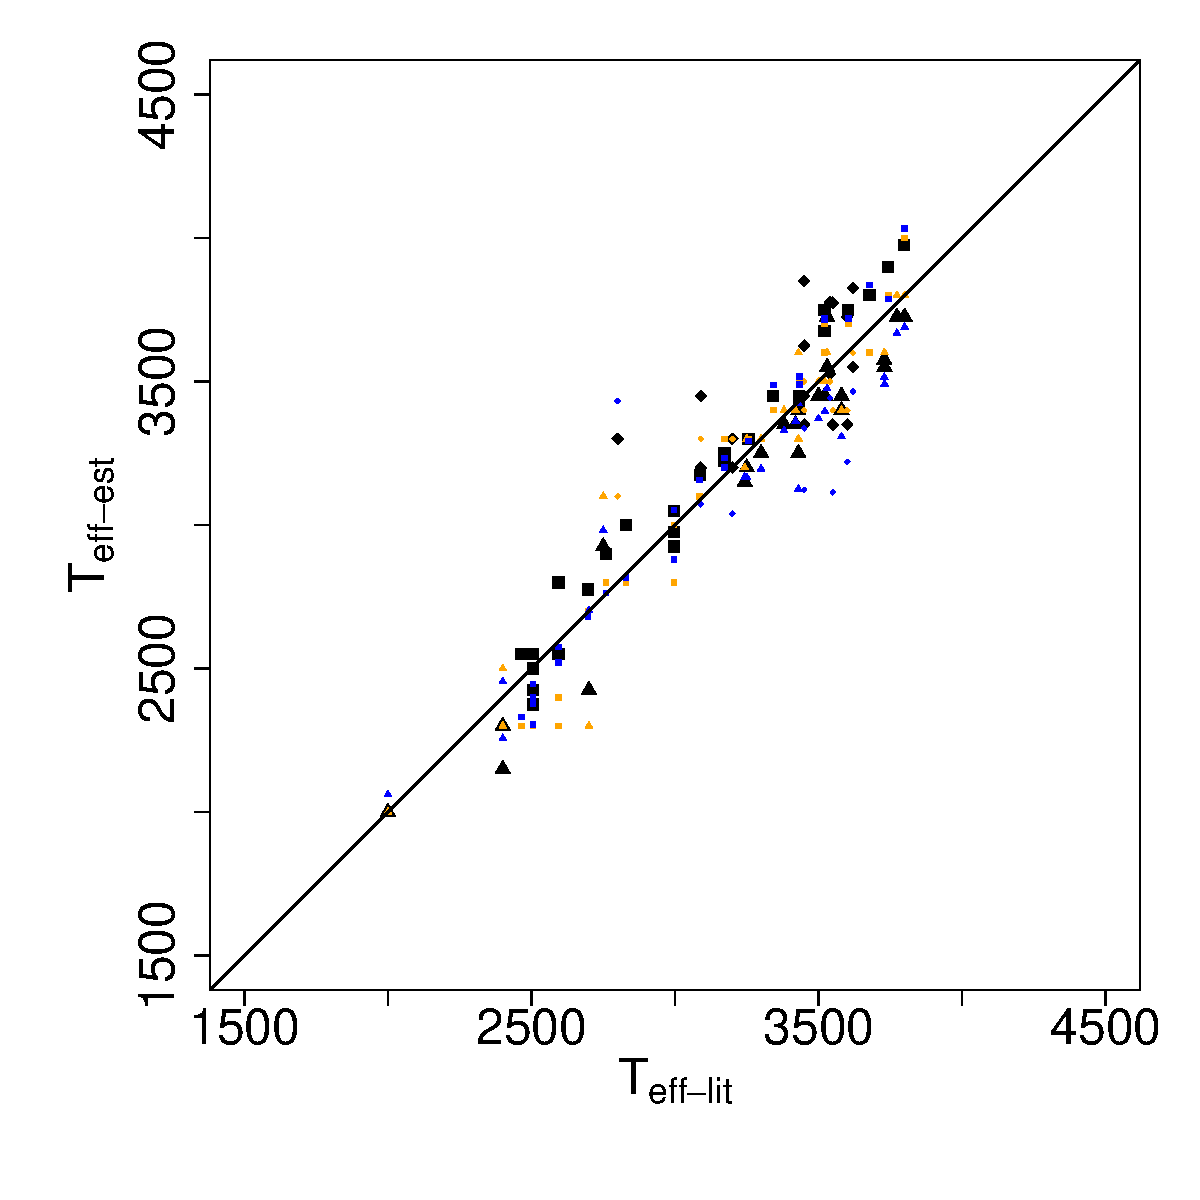
\includegraphics[scale=0.45]{figs/irtf-teffs-literature.pdf}
  
  \caption{Comparison of the effective temperatures from the
  literature included in \protect\cite{cesetti} and those inferred from the
  KNN module trained with the GA features (black). In orange and blue
  we show the estimates from the minimum $\chi^2$ estimate and from
  the PPR model based on the ICA components, respectively.}

\label{fig:irtf-teff}
\end {figure}

It is worth noting that in the M star regime, there are 63 effective
temperatures available in \cite{cesetti}, and 46 of the 63 were
estimated from the spectral types using the calibrations
of \cite{1996imsa.book.....O}. We have substituted them with a spline
fit to the combined datasets of M dwarfs in \cite{2013A&A...556A..15R}
and \cite{2012ApJ...757..112B} as it removes systematics in the
temperatures between 2500 and 3500 K.

It is not evident that the GA-KNN model performs significantly better
than the minimum $\chi^2$ estimate, but in the following we will
retain the former for further analysis. Figure \ref{fig:irtf-teff}
shows that the GA features can be used to estimate effective
temperatures with an accuracy equivalent to that yielded by full
wavelength range spectra of the same resolution.


%%%%%%%%%%%%%%%%%%%%%%%%%%%%%%%%%%%%%%%%%%%%%%%%%%%%%%%%%%%%%%
% TBD: Comparison with temperatures estimated with Cesetti features
%%%%%%%%%%%%%%%%%%%%%%%%%%%%%%%%%%%%%%%%%%%%%%%%%%%%%%%%%%%%%%

We have trained the same non linear regression models discussed above
using the features suggested by \cite{cesetti}. The performance of the
models based on these features are included in Table
\ref{tab:irtf-teff-rmse-cesetti}. From the comparison of Tables
\ref{tab:irtf-teff-rmse} and
\ref{tab:irtf-teff-rmse-cesetti} we can draw the following conclusions:

\begin{itemize}

\item The RMSE for SNR=10 and 50 is equivalent for the regression
  models trained on GA features and those recommended
  in \cite{cesetti};

\item However, the RMDSE from \cite{cesetti} is significantly higher
  in the case of the features for all SNR values.

\item In the unrealistic case of noiseless spectra, the features proposed
  by \cite{cesetti} produce RMSE and RMDSE significantly worse than
  the GA features.

\end{itemize}

However, the cross-validation errors are far from informative with
respect to the true performance when the models are applied to real
data. In the case of the features defined by \cite{cesetti}, we find
that the best RMSE/RMDSE (obtained not from cross-validation but from
the comparison with the effective temperatures in Table 3
of\cite{cesetti}) is attained by the CES-NNR
model. Figure \ref{fig:irtf-cesteff} shows the graphical comparison of
the CES-NNR predictions with the Table 3 reference values. Again, and
in the rest of this work, we substitute the effective temperatures in
that Table that were estimated using the \cite{1996imsa.book.....O}
calibration with those from the spline fit described above.

\begin {figure}
 \centering
  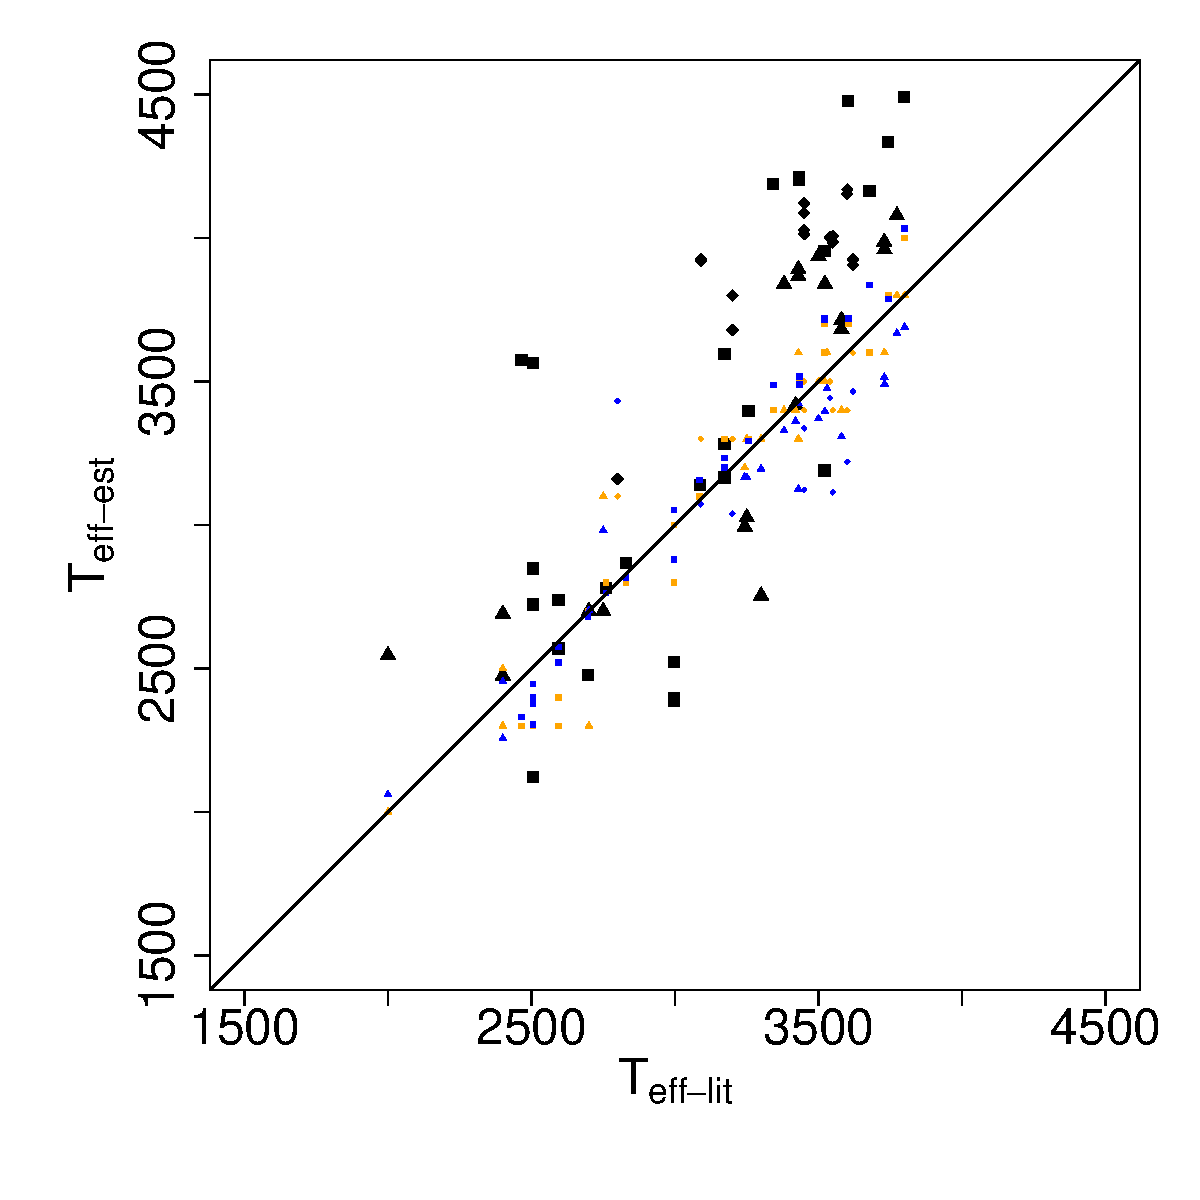
\includegraphics[scale=0.45]{figs/irtf-CESteffs-literature.pdf}
  
  \caption{Comparison of the effective temperatures from the
  literature included in \protect\cite{cesetti} and those inferred from the
  NNR module trained with the features introduced in \protect\cite{cesetti}
  (black). In orange and blue we show the estimates from the minimum
  $\chi^2$ estimate and from the PPR model based on the ICA
  components, respectively.}

\label{fig:irtf-cesteff}
\end {figure}

Figure \ref{fig:irtf-cesteff} shows that the features found by the GA
are to be prefered to the ones proposed by \cite{cesetti}. 

\subsubsection{Surface gravity models}

For the validation of our models, we only have 10 literature values of
the surface gravity available in Table 3 of
\cite{cesetti}. Unfortunately, this is too small figure to draw
significant conclusions on the comparison of methodologies from
external data. Hence, we are left only with plausibility arguments for
the selection of models. In this Section $\log(T_{\rm
eff})--\log(g)$ diagram comparisons will be used to select the most 
plausible model results. 

An important difference with respect to the models discussed
above is that we use the $T_{\rm eff}$ estimated in the previous stage
as input of our models. It introduces an average improvement in the
RMSE/RMDSE of 20\% with respect to the models without input
information on the effective temperature although it represents a risk
if the $T_{\rm eff}$ estimate is in gross error.

Table~\ref{tab:irtf-logg-rmse} shows the RMSE and RMDSE of the
cross-validation experiments for the $\log(g)$ regression models and
the same SNR regimes discussed for the estimation of $T_{\rm eff}$. We
have assessed the models according to plausibility arguments relative
to the distribution of the model predictions in $T_{\rm
eff}$--$\log(g)$ diagrams.  Figure~\ref{fig:lt_lg_ga} shows this
distribution for four models selected based on these plausibility
criteria: GA-RR, GA-PLS, GA-KNN (the three of them for SNR=50), and
PPR-ICA (clockwise, starting at the top left corner). All four panels
show a tendency towards lower surface gravities at the coolest end,
and a reasonable capability to separate dwarfs from giants, and giants
from supergiants. The estimates are in reasonable agreement with the
extrapolation of the distributions that can be guessed from the values
in Table 3 of \cite{cesetti} (represented with black filled
symbols). Since we cannot propose quantifications of this plausibility
argument, we let the reader decide which estimate (GA-RR, GA-PLS,
GA-KNN, or ICA-10) is to be prefered.

\begin{figure*}
 \begin{center}
   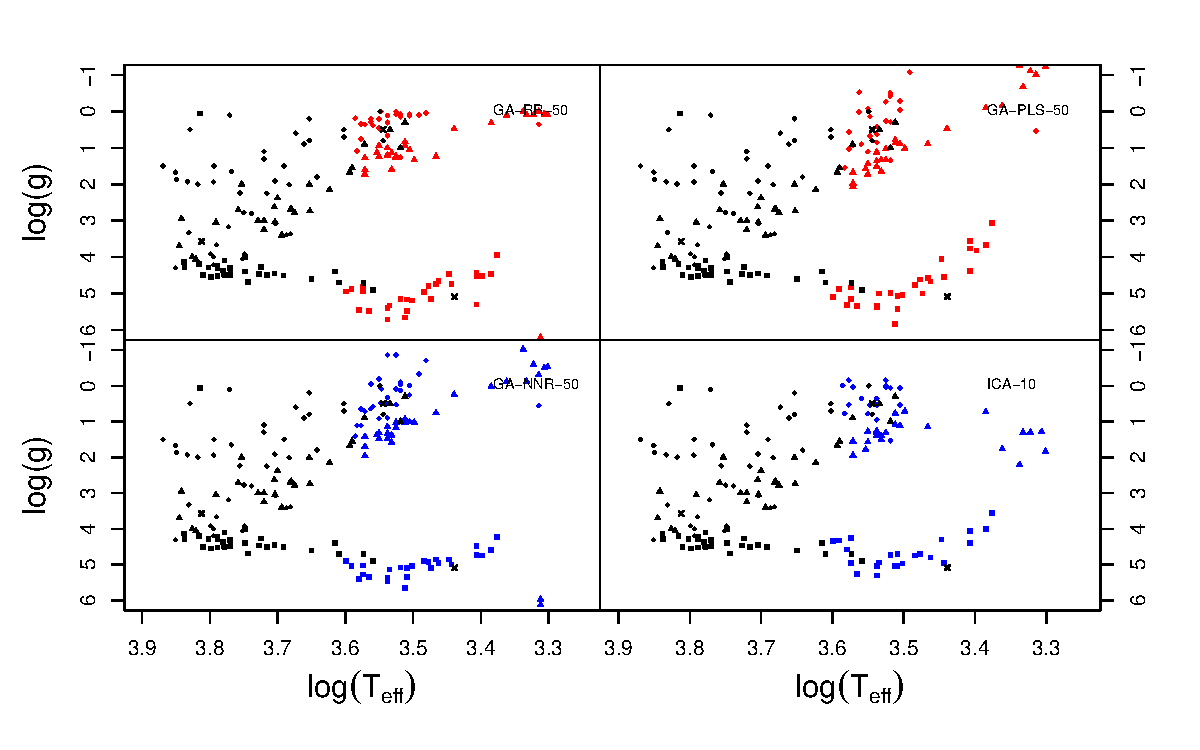
\includegraphics[width=\textwidth]{figs/ordieres-fig4.pdf}
\caption{$\log(T_{eff})$--$\log(g)$ diagrams produced by the GA-KNN
   (SNR=$\infty$) effective temperatures and gravities derived with
   the GA-RR (SNR=50), GA-PLS (SNR=50), GA-NNR (SNR=50), and
   $PPR-ICA-10$ models (clockwise, starting from the top left
   plot). Squares represent dwarfs stars, triangles represent
   luminosity class {\sc III} and circles represent luminosity classes
   {\sc I} and {\sc II}. Black symbols represent values taken
   from \protect\cite{cesetti} and red symbols are our own predictions.}

\label{fig:lt_lg_ga}
 \end{center}
\end{figure*}

Figure \ref{fig:irtf-ces} shows the equivalent diagram for predictions
obtained from the features selected in \cite{cesetti}. Again, we
select the regression models that yield the most plausible
$\log(T_{\rm eff})-\log(g)$ distributions with no quantitative
criteria defined to select the models. It is again evident the
superiority of the GA-based features over those defined
by \cite{cesetti}.

\subsubsection{Metallicity models} 
\label{sect:irtf-met}

Finally, the same machine learning models are trained to infer the
metallicity, again considering the effective temperature as an input
feature as in the $\log(g)$ regression
models. Table~\ref{tab:irtf-met-rmse} shows the RMSE and RMDSE
obtained for the cross-validation experiments of each regression
model. The minimum cross-validation errors are consistently obtained
with the minimum $\chi^2$, $PPR-ICA$ and $GA-KNN$ (with some
exceptions). The differences from these cross-validation experiments
are only marginal, but we see that even at these intermediate
resolutions the reduction of dimensionality (either with ICA or GA)
produces an improvement in the predictions. 

This is even more evident if we compare our predictions with more
recent metallicity estimates not included in \cite{cesetti}. We have
gathered estimates for stars in both the IRTF collection and a series
of recent metallicity catalogs
by \cite{RA2012}, \cite{NevesIII}, \cite{Newton2014}, \cite{Gaidos2015},
and \cite{Mann2015}. All of the aforementioned references provide us
with estimates of the iron abundance ratio [Fe/H] except \cite{RA2012}
that provides both the overall metallicity [M/H] and the [Fe/H]
ratio. Our estimates, coming from the BT-Settl library, are for the
[M/H] ratios, so some offset could be expected from the different
nature of the quantities compared. Hence, when comparing our estimates
with those from the literature, we compute the RMSE or RMDSE after
subtracting any difference in the mean. It turns out that, after
correcting for these different scales, $PPR-ICA$ trained with SNR=10
examples yields the lowest RMSE/RMDSE. Figure \ref{MIRTF_ICA_10}
represents the estimates of [M/H] obtained from the $PPR-ICA$ based
regressor, as a function of the values taken from these references for
the sources in common. 

The black empty circles represent values
from \cite{cesetti} ; orange filled circles, values
from \cite{NevesIII}; green filled squares, values that the Vizier
catalog entry for Table 8 of
\cite{NevesIII} links to \cite{Jao}. Although we find no evidence
that \cite{Jao} contains estimates of metallicities; cyan and blue
filled squares, are the values of [M/H] and [Fe/H] respectively
in \cite{RA2012}; red filled squares, values from \cite{Mann2015};
yellow filled squares, values from \cite{Newton2014}; and, finally,
black filles squares, values from \cite{Gaidos2015}.

It is remarkable that the minimum $\chi^2$ predictions result in a
50\% increase in the RMDSE with respect to the ICA-10 models and the
best performing GA-based models. Therefore, we advice against its use
in the context of metallicity estimations. 

 \begin{figure}
 \centering
 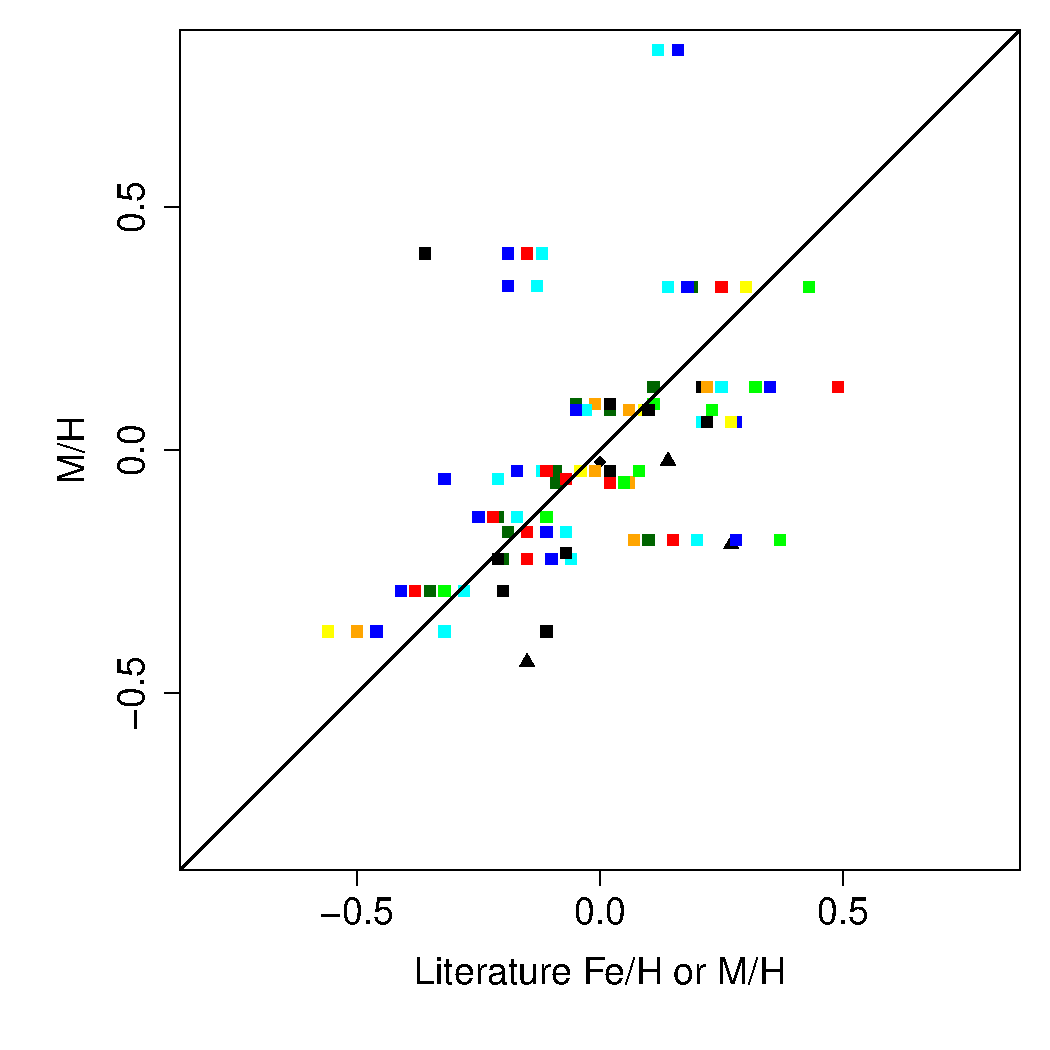
\includegraphics[width=0.45\textwidth]{figs/irtf-figs/M-ICA10.pdf}

\caption{Comparison
  between metallicity estimates from the literature and predictions
  from the PPR-ICA (SNR=10) model.  Black empty circles represent
  values from \protect\cite{cesetti} ; orange filled circles, values
  from \protect\cite{NevesIII}; green filled squares, values that the
  Vizier catalog entry for Table 8 of \protect\cite{NevesIII} links
  to \protect\cite{Jao}, although we find no evidence
  that \protect\cite{Jao} contains estimates of metallicities; cyan
  and blue filled squares, the values of [M/H] and [Fe/H] respectively
  in \protect\cite{RA2012}; red filled squares, values
  from \protect\cite{Mann2015}; yellow filled squares, values
  from \protect\cite{Newton2014}; and, finally, black filles squares, values
  from \protect\cite{Gaidos2015}.}

\label{MIRTF_ICA_10}
\end {figure}

Figure \ref{fig:irtf-teff-logg-met} summarizes the predictions from a
set of selected regression models in $T_{\rm eff}$ (from the
GA-NN-$\infty$ model), $\log(g)$ (from the GA-RR-50 model) and
metallicity (from the PPR-ICA-10 model). Again, plausibility arguments
such as the lower metallicity of the supergiants apparently give
evidence supporting the good performance of our models, but the lack
of extensive good-quality estimates of the physical parameters of the
IRTF collection of stars prevents us from a more quantitative
assessment of the predictions.

 \begin{figure}
 \centering
 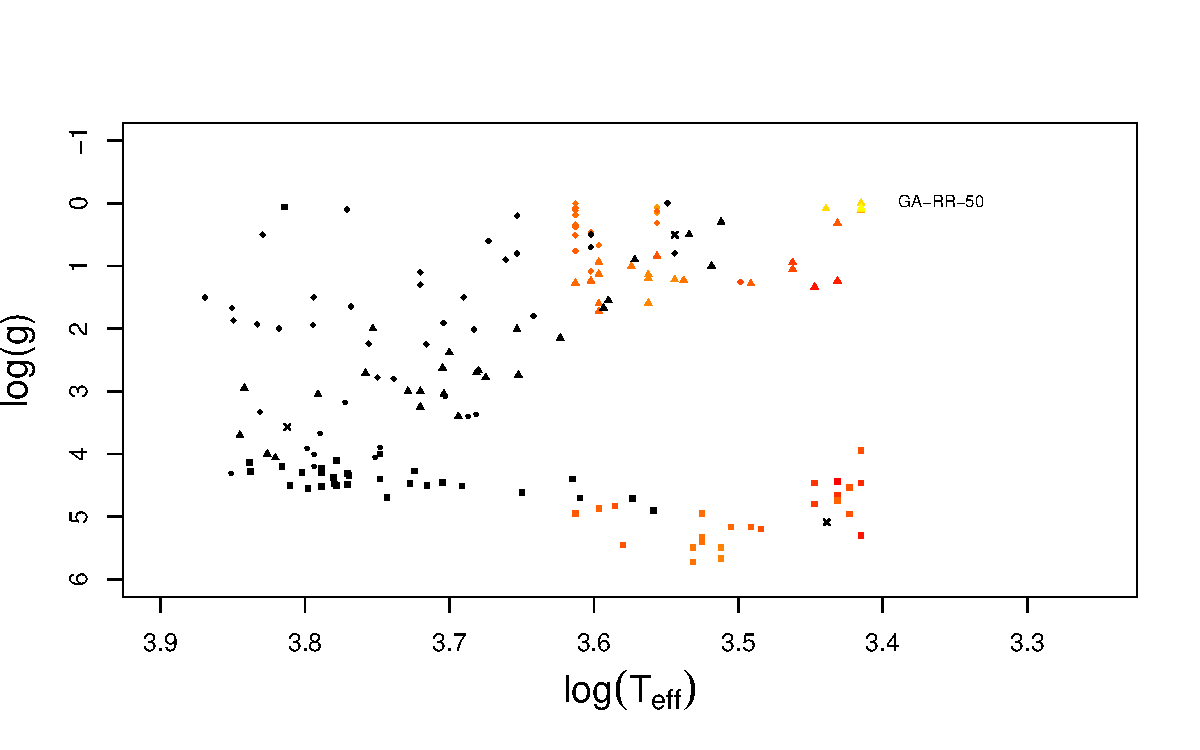
\includegraphics[width=0.5\textwidth]{figs/ordieres-fig8.pdf}
\caption{Plane of predictions for $T_{\rm eff}$ (from GA-KNN-$\infty$)
and $log(g)$ (from GA-RR-50) with metallicity predictions from
PPR-ICA-10.}
\label{fig:irtf-teff-logg-met}
\end {figure}

The equivalent plot for predictions based on the features defined
by \cite{cesetti} and the RF model trained with SNR=50 spectra is
included as Figure \ref{fig:irtf-ces-met}.


